% =============================================================================
% Simula Training Data Framework — Implementation Specification
% Style: Based on arabic-ap-spec.pdf (professional spec with TikZ, listings)
% =============================================================================
\documentclass[11pt,a4paper]{article}

% ─── Core packages ───────────────────────────────────────────────────────────
\usepackage[utf8]{inputenc}
\usepackage[T1]{fontenc}
\usepackage{lmodern}
\usepackage{amsmath}  % For \text in math mode
\usepackage[margin=2.5cm]{geometry}
\usepackage{graphicx}
\usepackage{booktabs}
\usepackage{longtable}
\usepackage{tabularx}
\usepackage{multirow}
\usepackage{array}
\usepackage{float}
\usepackage{enumitem}
\usepackage{xcolor}
\usepackage{hyperref}
\usepackage{fancyhdr}
\usepackage{titlesec}

% ─── Code listings ───────────────────────────────────────────────────────────
\usepackage{listings}

\definecolor{codebg}{RGB}{248,248,248}
\definecolor{codegreen}{RGB}{0,128,0}
\definecolor{codegray}{RGB}{128,128,128}
\definecolor{codeblue}{RGB}{0,0,180}
\definecolor{codepurple}{RGB}{128,0,128}

\lstdefinelanguage{Python}{
  keywords={class,def,return,if,elif,else,for,in,import,from,async,await,
            True,False,None,self,try,except,finally,with,as,yield,not,and,or,
            Optional,Dict,List,Tuple,Any,str,int,float,bool,dataclass,field,Enum},
  keywordstyle=\color{codeblue}\bfseries,
  sensitive=true,
  comment=[l]{\#},
  morecomment=[s]{"""}{"""},
  commentstyle=\color{codegreen}\itshape,
  stringstyle=\color{codepurple},
  morestring=[b]',
  morestring=[b]",
  backgroundcolor=\color{codebg},
}

\lstset{
  basicstyle=\ttfamily\small,
  breaklines=true,
  frame=single,
  numbers=left,
  numberstyle=\tiny\color{codegray},
  backgroundcolor=\color{codebg},
  captionpos=b,
}

% ─── TikZ for diagrams ───────────────────────────────────────────────────────
\usepackage{tikz}
\usetikzlibrary{arrows.meta,positioning,shapes.geometric,shapes.multipart,fit,calc}

% ─── SAP colors ──────────────────────────────────────────────────────────────
\definecolor{sapblue}{HTML}{0070F2}
\definecolor{sapgold}{HTML}{E78C07}
\definecolor{sapdark}{HTML}{354A5F}
\definecolor{saplight}{HTML}{F5F6F7}
\definecolor{hanagreen}{HTML}{00875A}
\definecolor{llmpurple}{HTML}{7B68EE}

% ─── Headers ─────────────────────────────────────────────────────────────────
\pagestyle{fancy}
\fancyhf{}
\fancyhead[L]{\small\color{sapdark}Simula Training Data Framework}
\fancyhead[R]{\small\color{sapdark}SAP OSS -- Studio AI}
\fancyfoot[C]{\thepage}
\renewcommand{\headrulewidth}{0.4pt}

\hypersetup{
    colorlinks=true,
    linkcolor=sapblue,
    urlcolor=sapblue,
    citecolor=sapblue
}

% ─── Title ───────────────────────────────────────────────────────────────────
\title{%
    \vspace{-1cm}
    {\LARGE\bfseries Reasoning-Driven Synthetic Training Data Generation}\\[0.3cm]
    {\Large for SAP HANA Cloud}\\[0.5cm]
    {\large Simula Framework: HANA-Direct Pipeline\\
    with vLLM TurboQuant}\\[0.3cm]
    {\normalsize Implementation Specification v1.0}\\[0.5cm]
    \rule{\textwidth}{1pt}
}
\author{%
    SAP OSS -- Studio AI\\
    \small Training Data Pipeline Working Group
}
\date{April 2026}

\begin{document}
\maketitle
\thispagestyle{empty}

% =============================================================================
% ABSTRACT
% =============================================================================
\begin{abstract}
\noindent
This specification defines the full implementation of the \textbf{Simula} reasoning-driven
synthetic training data generation framework for SAP HANA Cloud. The system addresses a
critical gap identified in the existing training pipeline: \emph{there is no direct pipe
to HANA to generate training datasets for model training}. Three orthogonal components
are specified in full:

\begin{itemize}[nosep]
    \item a \textbf{HANA Schema Extraction Pipeline} that connects to SAP HANA Cloud via
          the AI Core PAL MCP service, queries \texttt{SYS.TABLE\_COLUMNS} for live metadata,
          and populates a schema registry;
    \item a \textbf{Taxonomy Generation Engine} that implements Algorithm~1 from the Simula
          research paper---factor identification, breadth-first expansion with Best-of-N
          proposals, and generator-critic refinement;
    \item a \textbf{Training Data Generation Engine} that implements Algorithm~2---taxonomic
          mix sampling, meta-prompt generation, complexification, and double-critic filtering.
\end{itemize}

\noindent
All three components consume a single vLLM TurboQuant backend via the OpenAI-compatible API
and output JSONL training data suitable for LoRA fine-tuning. The specification targets
three application domains: Arabic document processing (invoice extraction), Trial Balance
review (variance analysis and LLM commentaries), and ESG analytics (financed emissions
classification).

\medskip
\noindent\textbf{Reading order.} Chapter~\ref{chap:overview} situates the work;
Chapter~\ref{chap:schema} defines the data structures; Chapter~\ref{chap:extraction}
covers the HANA extraction pipeline; Chapter~\ref{chap:taxonomy} covers the taxonomy
engine; Chapter~\ref{chap:generator} covers the data generator; Chapter~\ref{chap:config}
specifies environment and CLI; Chapter~\ref{chap:references} is a traceability appendix.

\medskip
\noindent\textbf{Conventions.} File paths are typeset in \texttt{monospace} and are
relative to the repository root \texttt{/Users/user/Documents/sap-oss}. Enum values
in running text appear in \textsc{small caps}. Python code listings include line numbers
for cross-reference.
\end{abstract}

\tableofcontents
\listoftables
\listoffigures
\newpage

% =============================================================================
% CHAPTER 1: OVERVIEW AND SCOPE
% =============================================================================
\section{Overview and Scope}
\label{chap:overview}

\subsection{The Problem}

The SAP OSS training pipeline requires high-quality Text-to-SQL training data that reflects
the actual schema structure of SAP HANA Cloud tables. The current implementation in
\texttt{src/training/pipeline/} uses metadata from \textbf{Excel files}
(\texttt{DATA\_DICTIONARY.xlsx}, \texttt{ESG\_DATA\_DICTIONARY.xlsx}) that were originally
exported from HANA or defined manually.

While the \texttt{HanaClient} in \texttt{src/training/pipeline/hana\_client.py} has the
capability to query \texttt{SYS.TABLE\_COLUMNS} for live schema metadata, this HANA-direct
extraction is \textbf{not currently integrated} into the main training data generation
pipeline.

\begin{table}[H]
\centering
\caption{Current vs. Target Training Data Pipeline}
\label{tab:gap-analysis}
\begin{tabularx}{\textwidth}{lXX}
\toprule
\textbf{Dimension} & \textbf{Current State} & \textbf{Target State} \\
\midrule
Schema Source & Static Excel/CSV files & Live HANA Cloud metadata \\
Extraction Method & Manual export & MCP-based automated query \\
Training Data & Template-based expansion & Reasoning-driven synthesis \\
Diversity Control & None & Taxonomic coverage \\
Quality Assurance & None & Double-critic filtering \\
Complexity Control & None & Calibrated Elo scoring \\
\bottomrule
\end{tabularx}
\end{table}

\subsection{Goals}

The specification targets three outcomes:

\begin{enumerate}[nosep]
    \item \textbf{HANA-Direct Extraction.} Every training dataset is generated from live
          schema metadata queried via the AI Core PAL MCP service.
    \item \textbf{Taxonomic Coverage.} The conceptual space of the target domain is mapped
          using hierarchical taxonomies, ensuring global diversity.
    \item \textbf{Reasoning-Driven Synthesis.} Each training example is generated from
          first principles using agentic refinement, ensuring quality, local diversity,
          and controlled complexity.
\end{enumerate}

\subsection{In-Scope Domains}

\begin{table}[H]
\centering
\caption{Application Domains}
\label{tab:domains}
\begin{tabularx}{\textwidth}{llX}
\toprule
\textbf{Domain} & \textbf{HANA Schema} & \textbf{Training Task} \\
\midrule
Arabic Document Processing & \texttt{AP\_INVOICES}, \texttt{VAT\_CHECKLISTS} & Invoice field extraction, VAT compliance \\
Trial Balance Review & \texttt{TB\_VARIANCES}, \texttt{GL\_BALANCES} & Variance analysis, commentary generation \\
ESG Analytics & \texttt{ESG\_METRICS}, \texttt{FINANCED\_EMISSIONS} & Scope classification, net-zero alignment \\
\bottomrule
\end{tabularx}
\end{table}

\subsection{System Context}

\begin{figure}[H]
\centering
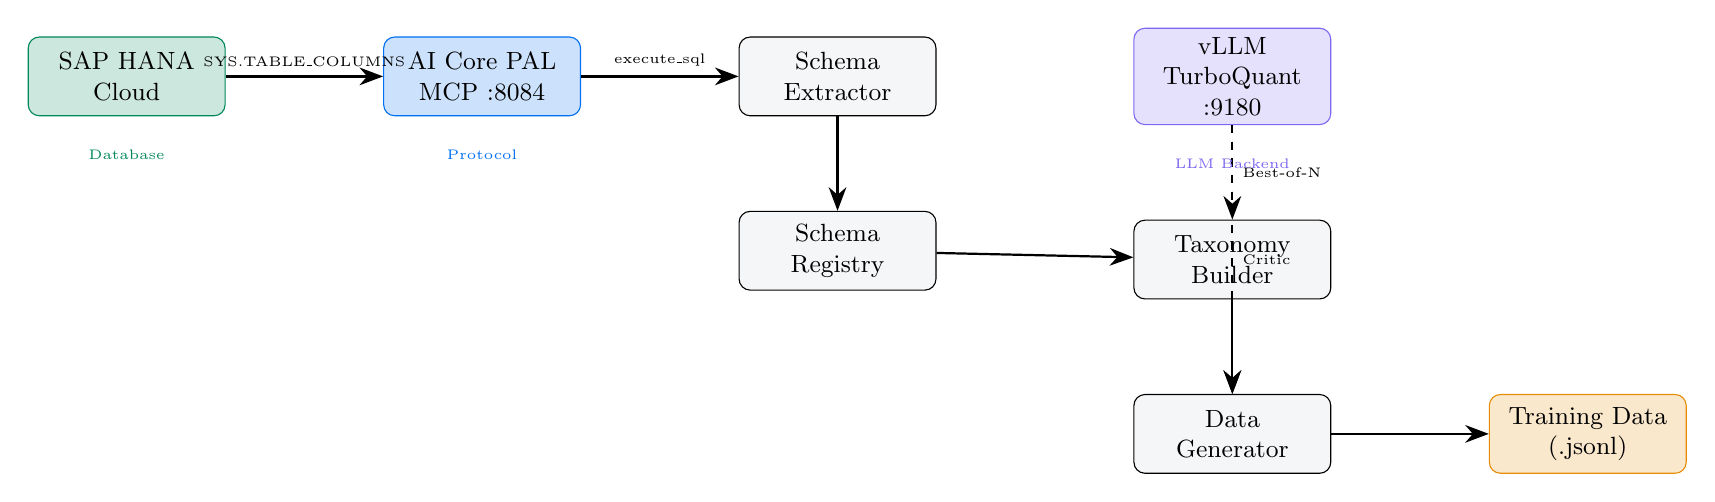
\begin{tikzpicture}[
    node distance=1.2cm and 2cm,
    box/.style={rectangle, draw, rounded corners, minimum width=2.5cm, minimum height=1cm, align=center, font=\small},
    hana/.style={box, fill=hanagreen!20, draw=hanagreen},
    mcp/.style={box, fill=sapblue!20, draw=sapblue},
    llm/.style={box, fill=llmpurple!20, draw=llmpurple},
    output/.style={box, fill=sapgold!20, draw=sapgold},
    arr/.style={-{Stealth[length=3mm]}, thick},
]
    % HANA Layer
    \node[hana] (hana) {SAP HANA\\Cloud};
    
    % MCP Layer
    \node[mcp, right=of hana] (mcp) {AI Core PAL\\MCP :8084};
    
    % Extraction
    \node[box, right=of mcp, fill=saplight] (extract) {Schema\\Extractor};
    
    % Registry
    \node[box, below=of extract, fill=saplight] (registry) {Schema\\Registry};
    
    % LLM
    \node[llm, right=2.5cm of extract] (llm) {vLLM\\TurboQuant\\:9180};
    
    % Taxonomy
    \node[box, below=of llm, fill=saplight] (taxonomy) {Taxonomy\\Builder};
    
    % Generator
    \node[box, below=of taxonomy, fill=saplight] (generator) {Data\\Generator};
    
    % Output
    \node[output, right=of generator] (output) {Training Data\\(.jsonl)};
    
    % Arrows
    \draw[arr] (hana) -- node[above, font=\tiny]{SYS.TABLE\_COLUMNS} (mcp);
    \draw[arr] (mcp) -- node[above, font=\tiny]{execute\_sql} (extract);
    \draw[arr] (extract) -- (registry);
    \draw[arr] (registry) -- (taxonomy);
    \draw[arr, dashed] (llm) -- node[right, font=\tiny]{Best-of-N} (taxonomy);
    \draw[arr] (taxonomy) -- (generator);
    \draw[arr, dashed] (llm) -- node[right, font=\tiny]{Critic} (generator);
    \draw[arr] (generator) -- (output);
    
    % Labels
    \node[below=0.3cm of hana, font=\tiny\color{hanagreen}] {Database};
    \node[below=0.3cm of mcp, font=\tiny\color{sapblue}] {Protocol};
    \node[below=0.3cm of llm, font=\tiny\color{llmpurple}] {LLM Backend};
\end{tikzpicture}
\caption{System context. HANA Cloud (green) provides live schema metadata via the MCP
protocol (blue). The vLLM backend (purple) powers taxonomy expansion and data generation.
Output is JSONL training data (gold).}
\label{fig:system-context}
\end{figure}

\subsection{Out of Scope}

The following are \textbf{explicitly} out of scope for this document:

\begin{itemize}[nosep]
    \item Model fine-tuning and evaluation (covered by separate LoRA training specification).
    \item Downstream inference and routing (covered by \texttt{03-prompt-routing.tex}).
    \item Trial Balance business process (covered by \texttt{04-trial-balance-ai-specification.tex}).
    \item Arabic invoice pipeline (covered by the Arabic AP specification).
\end{itemize}

% =============================================================================
% CHAPTER 2: CANONICAL DATA SCHEMA
% =============================================================================
\newpage
\section{Canonical Data Schema}
\label{chap:schema}

\subsection{Layout of \texttt{src/training/pipeline/}}

\begin{table}[H]
\centering
\caption{Pipeline Module Layout}
\label{tab:module-layout}
\begin{tabularx}{\textwidth}{lX}
\toprule
\textbf{Path} & \textbf{Purpose} \\
\midrule
\texttt{simula\_config.py} & Configuration dataclasses for all components \\
\texttt{simula\_llm\_client.py} & OpenAI-compatible async LLM client \\
\texttt{hana\_schema\_extractor.py} & HANA Cloud schema extraction via MCP \\
\texttt{simula\_taxonomy\_builder.py} & Algorithm 1: Taxonomy generation \\
\texttt{simula\_data\_generator.py} & Algorithm 2: Training data synthesis \\
\texttt{schema\_registry.py} & In-memory schema registry \\
\bottomrule
\end{tabularx}
\end{table}

\subsection{Training Example Record}

Each generated training example is a JSON object with the following structure:

\begin{lstlisting}[language=Python,caption={TrainingExample dataclass (simula\_data\_generator.py)}]
@dataclass
class TrainingExample:
    """A single training example for Text-to-SQL."""
    id: str                    # Unique identifier
    question: str              # Natural language question
    sql: str                   # Target SQL query
    schema_context: str        # Table/column descriptions
    taxonomy_path: list[str]   # Factor nodes used
    complexity_score: float    # 0.0 to 1.0
    meta_prompt: str           # The meta-prompt used
    is_complexified: bool      # Whether complexification applied
    critic_passed: bool        # Whether double-critic passed
    generation_metadata: dict  # Timestamps, model, etc.
\end{lstlisting}

\subsection{Schema Registry}

The \texttt{SchemaRegistry} holds table and column metadata extracted from HANA:

\begin{lstlisting}[language=Python,caption={Schema registry structures (schema\_registry.py)}]
@dataclass
class Column:
    name: str
    data_type: str
    length: int | None
    nullable: bool
    description: str = ""

@dataclass
class TableSchema:
    schema_name: str
    table_name: str
    columns: list[Column]
    primary_key: list[str] = field(default_factory=list)
    description: str = ""
\end{lstlisting}

\subsection{Taxonomy Structure}

Taxonomies are hierarchical trees where each node represents a factor of variation:

\begin{lstlisting}[language=Python,caption={Taxonomy structures (simula\_taxonomy\_builder.py)}]
@dataclass
class TaxonomyNode:
    id: str
    name: str
    description: str
    level: int
    parent_id: str | None
    children: list["TaxonomyNode"]
    examples: list[str]  # Sample values

@dataclass
class Factor:
    id: str
    name: str
    description: str
    taxonomy: "Taxonomy"

@dataclass
class Taxonomy:
    id: str
    factor: str
    root: TaxonomyNode
    depth: int
    total_nodes: int
\end{lstlisting}

\subsection{Enumerations}

\begin{table}[H]
\centering
\caption{Key Enumerations}
\label{tab:enums}
\begin{tabular}{lll}
\toprule
\textbf{Enum} & \textbf{Values} & \textbf{Description} \\
\midrule
\texttt{LLMProvider} & \textsc{vllm}, \textsc{openai}, \textsc{anthropic} & LLM backend type \\
\texttt{SamplingStrategy} & \textsc{uniform}, \textsc{weighted}, \textsc{coverage} & How to sample taxonomy nodes \\
\bottomrule
\end{tabular}
\end{table}

% =============================================================================
% CHAPTER 3: HANA SCHEMA EXTRACTION PIPELINE
% =============================================================================
\newpage
\section{HANA Schema Extraction Pipeline}
\label{chap:extraction}

\subsection{Pipeline at a Glance}

\begin{figure}[H]
\centering
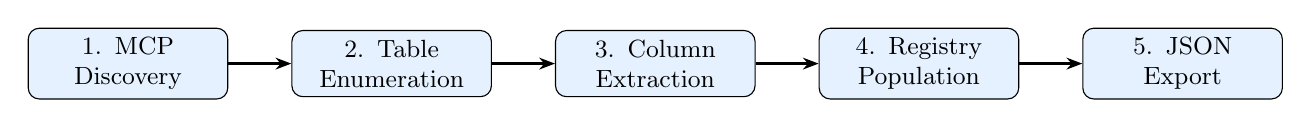
\begin{tikzpicture}[
    node distance=0.8cm,
    stage/.style={rectangle, draw, rounded corners, fill=sapblue!10, 
                  minimum width=2.5cm, minimum height=0.8cm, font=\small,
                  text width=2.3cm, align=center},
    arr/.style={-{Stealth[length=2mm]}, thick},
]
    \node[stage] (s1) {1. MCP Discovery};
    \node[stage, right=of s1] (s2) {2. Table Enumeration};
    \node[stage, right=of s2] (s3) {3. Column Extraction};
    \node[stage, right=of s3] (s4) {4. Registry Population};
    \node[stage, right=of s4] (s5) {5. JSON Export};
    
    \draw[arr] (s1) -- (s2);
    \draw[arr] (s2) -- (s3);
    \draw[arr] (s3) -- (s4);
    \draw[arr] (s4) -- (s5);
\end{tikzpicture}
\caption{The five extraction stages; each emits a well-typed payload to the next.}
\label{fig:extraction-pipeline}
\end{figure}

\subsection{Stage 1 --- MCP Discovery}

The extractor connects to the AI Core PAL MCP server and discovers available tools:

\begin{lstlisting}[language=Python,caption={MCP connection (hana\_schema\_extractor.py, lines 45--60)}]
async def connect(self) -> None:
    """Establish MCP connection to AI Core PAL."""
    transport_url = self.config.mcp_url.replace("http://", "ws://")
    transport_url = f"{transport_url}/mcp/ws"
    
    self._transport = WebSocketClientTransport(transport_url)
    self._session = ClientSession(self._transport)
    
    await self._session.initialize()
    
    # Discover available tools
    tools_result = await self._session.list_tools()
    self._available_tools = {t.name for t in tools_result.tools}
\end{lstlisting}

\textbf{Precondition.} The MCP server must expose at least one of: \texttt{execute\_sql},
\texttt{hana\_tables}, or \texttt{list\_tables}.

\subsection{Stage 2 --- Table Enumeration}

Tables are discovered via the \texttt{hana\_tables} MCP tool or by querying
\texttt{SYS.TABLES}:

\begin{lstlisting}[language=Python,caption={Table discovery (hana\_schema\_extractor.py, lines 85--105)}]
async def _discover_tables(self, schema: str) -> list[str]:
    """Discover tables in a schema."""
    if "hana_tables" in self._available_tools:
        result = await self._session.call_tool(
            "hana_tables",
            {"schema": schema}
        )
        return [t["table_name"] for t in result.content]
    else:
        # Fallback to direct SQL
        result = await self._execute_sql(
            'SELECT TABLE_NAME FROM SYS.TABLES '
            'WHERE SCHEMA_NAME = ?',
            [schema]
        )
        return [row["TABLE_NAME"] for row in result]
\end{lstlisting}

\subsection{Stage 3 --- Column Extraction}

For each table, column metadata is extracted from \texttt{SYS.TABLE\_COLUMNS}:

\begin{lstlisting}[language=Python,caption={Column extraction SQL}]
SELECT 
    COLUMN_NAME,
    DATA_TYPE_NAME,
    LENGTH,
    IS_NULLABLE
FROM SYS.TABLE_COLUMNS
WHERE SCHEMA_NAME = ? AND TABLE_NAME = ?
ORDER BY POSITION
\end{lstlisting}

\subsection{Stage 4 --- Registry Population}

Extracted metadata is normalized and stored in the \texttt{SchemaRegistry}:

\begin{lstlisting}[language=Python,caption={Registry population (hana\_schema\_extractor.py, lines 140--165)}]
async def extract_table_schema(
    self, schema: str, table: str
) -> TableSchema:
    """Extract full schema for a single table."""
    columns_data = await self._get_table_columns(schema, table)
    
    columns = [
        Column(
            name=col["COLUMN_NAME"],
            data_type=col["DATA_TYPE_NAME"],
            length=col.get("LENGTH"),
            nullable=col.get("IS_NULLABLE", "TRUE") == "TRUE",
        )
        for col in columns_data
    ]
    
    return TableSchema(
        schema_name=schema,
        table_name=table,
        columns=columns,
    )
\end{lstlisting}

\subsection{Stage 5 --- JSON Export}

The registry exports to JSON for caching and debugging:

\begin{lstlisting}[language=Python,caption={JSON export format}]
{
  "schemas": {
    "PAL_STORE": {
      "tables": {
        "ESG_METRICS": {
          "columns": [
            {"name": "METRIC_ID", "type": "INTEGER", ...},
            {"name": "SCOPE", "type": "NVARCHAR", ...}
          ]
        }
      }
    }
  },
  "extracted_at": "2026-04-18T08:00:00Z"
}
\end{lstlisting}

% =============================================================================
% CHAPTER 4: TAXONOMY GENERATION ENGINE
% =============================================================================
\newpage
\section{Taxonomy Generation Engine}
\label{chap:taxonomy}

\subsection{Algorithm 1: Reasoning-Driven Taxonomy Generation}

The taxonomy builder implements Algorithm~1 from the Simula research paper. Given a
dataset description $y$ and target depth $D$, it produces a set of taxonomies
$\mathcal{T} = \{T_i\}_{i=0}^{K}$ that map the conceptual space.

\begin{figure}[H]
\centering
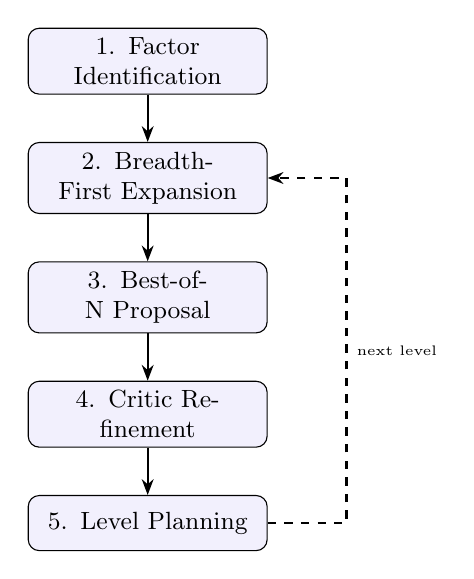
\begin{tikzpicture}[
    node distance=0.6cm and 1.5cm,
    stepbox/.style={rectangle, draw, rounded corners, fill=llmpurple!10,
                 minimum width=3cm, minimum height=0.7cm, font=\small,
                 text width=2.8cm, align=center},
    arr/.style={-{Stealth[length=2mm]}, thick},
]
    \node[stepbox] (f1) {1. Factor Identification};
    \node[stepbox, below=of f1] (f2) {2. Breadth-First Expansion};
    \node[stepbox, below=of f2] (f3) {3. Best-of-N Proposal};
    \node[stepbox, below=of f3] (f4) {4. Critic Refinement};
    \node[stepbox, below=of f4] (f5) {5. Level Planning};
    
    \draw[arr] (f1) -- (f2);
    \draw[arr] (f2) -- (f3);
    \draw[arr] (f3) -- (f4);
    \draw[arr] (f4) -- (f5);
    \draw[arr, dashed] (f5.east) -- ++(1,0) |- node[right, pos=0.25, font=\tiny]{next level} (f2.east);
\end{tikzpicture}
\caption{Taxonomy generation stages with iterative refinement.}
\label{fig:taxonomy-stages}
\end{figure}

\subsection{Step 1: Factor Identification}

Given schema metadata, the LLM proposes factors of variation:

\begin{lstlisting}[language=Python,caption={Factor identification prompt}]
SYSTEM: You identify the prime factors of variation for a 
        Text-to-SQL training dataset.
        
USER:   Schema context:
        {schema_context}
        
        Identify 3-7 factors that capture the main dimensions
        of queries users might ask. Examples:
        - "query_complexity" (simple, join, aggregation, subquery)
        - "time_range" (point-in-time, period, YTD, MTD)
        - "entity_type" (customer, order, product, supplier)
        
        Output JSON: {"factors": [{"name": "...", "description": "..."}]}
\end{lstlisting}

\subsection{Step 2: Breadth-First Expansion}

Each factor is expanded into a taxonomy tree. For each node, the LLM proposes children:

\begin{lstlisting}[language=Python,caption={Node expansion (simula\_taxonomy\_builder.py, lines 180--220)}]
async def _expand_node(
    self, node: TaxonomyNode, context: str
) -> list[TaxonomyNode]:
    """Expand a single node with Best-of-N proposals."""
    
    # Step 1: Generate N proposals
    proposals = await self.llm.best_of_n(
        prompt=self._build_expansion_prompt(node, context),
        n=self.config.taxonomy.best_of_n,
        temperature=0.8,
    )
    
    # Merge proposals into candidate set
    candidates = self._merge_proposals(proposals)
    
    # Step 2: Critic refinement
    refined = await self._critic_refine(node, candidates, context)
    
    return refined
\end{lstlisting}

\subsection{Step 3: Best-of-N Proposal}

Multiple proposals are generated to increase coverage:

\begin{lstlisting}[language=Python,caption={Best-of-N sampling}]
async def best_of_n(
    self,
    prompt: str,
    n: int = 5,
    temperature: float = 0.8,
) -> list[str]:
    """Generate N diverse completions."""
    tasks = [
        self.generate(prompt, temperature=temperature)
        for _ in range(n)
    ]
    responses = await asyncio.gather(*tasks)
    return [r.content for r in responses]
\end{lstlisting}

\subsection{Step 4: Critic Refinement}

The critic evaluates and refines the proposed children:

\begin{lstlisting}[language=Python,caption={Critic refinement prompt}]
SYSTEM: You are a taxonomy critic. Evaluate the proposed children
        for COMPLETENESS, SOUNDNESS, and SPECIFICITY.
        
USER:   Parent node: {parent.name} - {parent.description}
        Siblings: {siblings}
        Proposed children: {candidates}
        
        Actions you may take:
        - ADD: missing concepts
        - REMOVE: irrelevant or duplicate nodes
        - MERGE: overlapping concepts
        - EDIT: improve descriptions
        
        Output JSON with refined children list.
\end{lstlisting}

\subsection{Step 5: Level Planning}

After completing a level, a plan is generated for the next level:

\begin{lstlisting}[language=Python,caption={Level planning}]
async def _plan_next_level(
    self, current_level_nodes: list[TaxonomyNode]
) -> str:
    """Generate guidance for next level expansion."""
    prompt = f"""
    Current level nodes: {[n.name for n in current_level_nodes]}
    
    Generate a plan for expanding the next level that ensures:
    1. Consistent granularity across all branches
    2. No overlap between sibling expansions
    3. Complete coverage of the concept space
    """
    response = await self.llm.generate(prompt)
    return response.content
\end{lstlisting}

\subsection{Worked Example: Trial Balance Taxonomy}

\begin{table}[H]
\centering
\caption{Sample Taxonomy for Trial Balance Domain}
\label{tab:tb-taxonomy}
\begin{tabular}{llll}
\toprule
\textbf{Level 0} & \textbf{Level 1} & \textbf{Level 2} & \textbf{Level 3} \\
\midrule
query\_type & aggregation & sum & by\_account \\
            &             &     & by\_department \\
            &             & count & distinct\_accounts \\
            & comparison & variance & MoM \\
            &            &          & YoY \\
            & filter & by\_threshold & exceeds\_100M \\
\bottomrule
\end{tabular}
\end{table}

% =============================================================================
% CHAPTER 5: TRAINING DATA GENERATION ENGINE
% =============================================================================
\newpage
\section{Training Data Generation Engine}
\label{chap:generator}

\subsection{Algorithm 2: Agentic Data Synthesis}

Given taxonomies $\mathcal{T}$ and a target size $N$, the generator produces a synthetic
dataset optimized for diversity, complexity, and quality.

\begin{figure}[H]
\centering
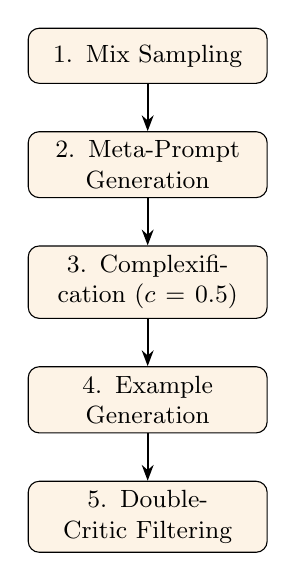
\begin{tikzpicture}[
    node distance=0.6cm and 1.5cm,
    stepbox/.style={rectangle, draw, rounded corners, fill=sapgold!10,
                 minimum width=3cm, minimum height=0.7cm, font=\small,
                 text width=2.8cm, align=center},
    arr/.style={-{Stealth[length=2mm]}, thick},
]
    \node[stepbox] (s1) {1. Mix Sampling};
    \node[stepbox, below=of s1] (s2) {2. Meta-Prompt Generation};
    \node[stepbox, below=of s2] (s3) {3. Complexification ($c=0.5$)};
    \node[stepbox, below=of s3] (s4) {4. Example Generation};
    \node[stepbox, below=of s4] (s5) {5. Double-Critic Filtering};
    
    \draw[arr] (s1) -- (s2);
    \draw[arr] (s2) -- (s3);
    \draw[arr] (s3) -- (s4);
    \draw[arr] (s4) -- (s5);
\end{tikzpicture}
\caption{Data generation stages implementing Algorithm 2.}
\label{fig:generator-stages}
\end{figure}

\subsection{Step 1: Mix Sampling (Global Diversity)}

Nodes are sampled from taxonomies to create ``mixes''---combinations of factors:

\begin{lstlisting}[language=Python,caption={Mix sampling (simula\_data\_generator.py, lines 120--150)}]
def _sample_mix(
    self, taxonomies: list[Taxonomy], strategy: SamplingStrategy
) -> list[TaxonomyNode]:
    """Sample a mix of nodes from taxonomies."""
    mix = []
    for taxonomy in taxonomies:
        if strategy == SamplingStrategy.UNIFORM:
            # Sample uniformly from leaf nodes
            leaves = self._get_leaf_nodes(taxonomy.root)
            node = random.choice(leaves)
        elif strategy == SamplingStrategy.COVERAGE:
            # Prioritize under-sampled nodes
            node = self._get_least_sampled_node(taxonomy)
        mix.append(node)
    return mix
\end{lstlisting}

\subsection{Step 2: Meta-Prompt Generation (Local Diversity)}

Each mix is converted to a meta-prompt that guides example generation:

\begin{lstlisting}[language=Python,caption={Meta-prompt generation}]
async def _generate_meta_prompt(
    self, mix: list[TaxonomyNode], schema_context: str
) -> str:
    """Generate a meta-prompt from a taxonomy mix."""
    prompt = f"""
    Generate a natural language question that a user might ask,
    given these requirements:
    
    {self._format_mix(mix)}
    
    Schema context:
    {schema_context}
    
    The question should be realistic and answerable with SQL.
    """
    response = await self.llm.generate(prompt, temperature=0.9)
    return response.content
\end{lstlisting}

\subsection{Step 3: Complexification}

A fraction $c$ (default 0.5) of examples undergo complexification:

\begin{lstlisting}[language=Python,caption={Complexification prompt}]
SYSTEM: You increase the complexity of a Text-to-SQL example
        while maintaining correctness.
        
USER:   Original question: {question}
        Original SQL: {sql}
        
        Add complexity by:
        - Adding edge cases or constraints
        - Requiring additional joins
        - Adding subqueries or CTEs
        - Handling NULL values explicitly
        
        Output the complexified question and SQL.
\end{lstlisting}

\subsection{Step 4: Example Generation}

The meta-prompt is used to generate a complete training example:

\begin{lstlisting}[language=Python,caption={Example generation}]
async def _generate_example(
    self, meta_prompt: str, schema_context: str
) -> TrainingExample:
    """Generate a single training example."""
    prompt = f"""
    Generate a Text-to-SQL training example.
    
    Meta-prompt: {meta_prompt}
    Schema: {schema_context}
    
    Output JSON:
    {{
      "question": "...",
      "sql": "SELECT ..."
    }}
    """
    response = await self.llm.generate(prompt)
    return self._parse_example(response.content)
\end{lstlisting}

\subsection{Step 5: Double-Critic Filtering}

The double-critic mitigates sycophancy bias by independently querying correctness
and incorrectness:

\begin{lstlisting}[language=Python,caption={Double-critic evaluation (simula\_llm\_client.py, lines 180--220)}]
async def double_critic_evaluate(
    self, question: str, sql: str, schema: str
) -> tuple[bool, str]:
    """Evaluate with double-critic to mitigate sycophancy."""
    
    # Query 1: Is this correct?
    correct_response = await self.generate(
        f"Is this SQL correct for the question?\n"
        f"Question: {question}\n"
        f"SQL: {sql}\n"
        f"Schema: {schema}\n"
        f"Answer YES or NO with explanation."
    )
    
    # Query 2: Is this incorrect?
    incorrect_response = await self.generate(
        f"Is this SQL INCORRECT for the question?\n"
        f"Question: {question}\n"
        f"SQL: {sql}\n"
        f"Schema: {schema}\n"
        f"Answer YES or NO with explanation."
    )
    
    # Accept only if: correct=YES AND incorrect=NO
    is_valid = (
        "YES" in correct_response.content.upper() and
        "NO" in incorrect_response.content.upper()
    )
    
    return is_valid, f"{correct_response.content}\n---\n{incorrect_response.content}"
\end{lstlisting}

\subsection{Output Format}

Generated examples are written to JSONL:

\begin{lstlisting}[language=Python,caption={JSONL output format}]
{"id": "sim-001", "question": "What is the total revenue...", 
 "sql": "SELECT SUM(amount) FROM...", "complexity_score": 0.3, ...}
{"id": "sim-002", "question": "Show all customers with...", 
 "sql": "SELECT * FROM customers WHERE...", "complexity_score": 0.7, ...}
\end{lstlisting}

% =============================================================================
% CHAPTER 6: ENVIRONMENT AND CLI
% =============================================================================
\newpage
\section{Environment and CLI}
\label{chap:config}

\subsection{Configuration Table}

\begin{longtable}{p{5cm}p{3cm}p{6cm}}
\caption{Environment Variables} \\
\toprule
\textbf{Variable} & \textbf{Default} & \textbf{Description} \\
\midrule
\endfirsthead
\toprule
\textbf{Variable} & \textbf{Default} & \textbf{Description} \\
\midrule
\endhead
\texttt{AICORE\_PAL\_MCP\_URL} & \texttt{http://localhost:8084} & AI Core PAL MCP endpoint \\
\texttt{VLLM\_BASE\_URL} & \texttt{http://localhost:9180/v1} & vLLM TurboQuant endpoint \\
\texttt{VLLM\_MODEL} & \texttt{Qwen/Qwen3.5-35B} & Model for generation \\
\texttt{SIMULA\_TARGET\_COUNT} & \texttt{100000} & Target training examples \\
\texttt{SIMULA\_COMPLEXITY\_RATIO} & \texttt{0.5} & Fraction to complexify \\
\texttt{SIMULA\_TAXONOMY\_DEPTH} & \texttt{4} & Max taxonomy depth \\
\texttt{SIMULA\_BEST\_OF\_N} & \texttt{5} & Proposals per expansion \\
\texttt{SIMULA\_ENABLE\_CRITIC} & \texttt{true} & Enable double-critic \\
\texttt{SIMULA\_OUTPUT\_DIR} & \texttt{data/training/} & Output directory \\
\bottomrule
\end{longtable}

\subsection{CLI Usage}

\begin{lstlisting}[language=bash,caption={CLI entry point}]
# Basic usage
python src/training/scripts/run_hana_pipeline.py

# Full customization
python src/training/scripts/run_hana_pipeline.py \
    --hana-schemas PAL_STORE,ESG_METRICS \
    --llm-url http://localhost:9180/v1 \
    --target-count 50000 \
    --complexity-ratio 0.5 \
    --taxonomy-depth 4 \
    --output data/training/

# Schema extraction only
python src/training/scripts/run_hana_pipeline.py \
    --extract-only \
    --output schemas/
\end{lstlisting}

\subsection{Output Files}

\begin{table}[H]
\centering
\caption{Pipeline Output Files}
\label{tab:outputs}
\begin{tabularx}{\textwidth}{lX}
\toprule
\textbf{File} & \textbf{Description} \\
\midrule
\texttt{schemas.json} & Extracted HANA schema metadata \\
\texttt{taxonomies.json} & Generated taxonomy trees \\
\texttt{training\_data.jsonl} & Final training examples \\
\texttt{generation\_stats.json} & Statistics (counts, rates, timing) \\
\texttt{rejected\_examples.jsonl} & Examples that failed critic \\
\texttt{complexity\_elo\_scores.json} & Elo-calibrated complexity scores \\
\texttt{coverage\_report.json} & Taxonomic coverage metrics \\
\texttt{diversity\_metrics.json} & Global + local diversity \\
\texttt{critic\_calibration.json} & Critic validation results \\
\bottomrule
\end{tabularx}
\end{table}

% =============================================================================
% CHAPTER 7: EVALUATION FRAMEWORK
% =============================================================================
\newpage
\section{Evaluation Framework}
\label{chap:evaluation}

This section specifies the evaluation components required for Simula methodology
compliance, as described in Sections 2.3, 3.1, and 3.3 of the research paper.

\subsection{Calibrated Complexity Scoring (Algorithm 3)}

Raw per-sample complexity scores are noisy due to model overconfidence.
The complexity calibrator uses batch-wise relative scoring with Elo ranking:

\begin{lstlisting}[language=Python,caption={Complexity calibrator usage}]
from src.training.pipeline import (
    SimulaComplexityCalibrator,
    ComplexityConfig,
)

calibrator = SimulaComplexityCalibrator(
    llm_client=llm,
    config=ComplexityConfig(
        batch_size=5,   # BS=5 from Figure 10
        n_samples=5,    # N=5 from Figure 10
        enable_elo=True,
    ),
)

# Calibrate all examples
scores = await calibrator.calibrate(examples)

# Split by complexity (Figure 7)
low, mid, high = calibrator.split_by_complexity(
    examples,
    low_percentile=0.4,
    high_percentile=0.6,
)

# Export scores
calibrator.export_scores("complexity_elo_scores.json")
\end{lstlisting}

\textbf{Key insight from paper:} High-complexity data yields +10\% accuracy on GSM8k
at 64k samples (Figure 7), but can \emph{hurt} performance when the teacher model
is weak (LEXam case).

\subsection{Taxonomic Coverage Evaluation}

The coverage evaluator measures Level Ratio Coverage---the proportion of unique
taxonomy nodes covered at each level:

\begin{lstlisting}[language=Python,caption={Coverage evaluator usage}]
from src.training.pipeline import (
    SimulaCoverageEvaluator,
    CoverageConfig,
    identify_coverage_gaps,
)

evaluator = SimulaCoverageEvaluator(
    llm_client=llm,
    config=CoverageConfig(
        max_level=4,
        sample_size=1000,
    ),
)

# Evaluate against all taxonomies
reports = await evaluator.evaluate_multiple(examples, taxonomies)

# Identify gaps
gaps = identify_coverage_gaps(reports, threshold=0.5)
print(f"Under-covered nodes: {gaps}")

# Export
evaluator.export_all_reports(reports, "coverage_report.json")
\end{lstlisting}

\subsection{Embedding-Based Diversity Metrics}

Following Yu et al. (2023), diversity is measured via cosine distance in embedding
space. \textbf{Global diversity} is the average pairwise distance across the dataset.
\textbf{Local diversity} is the average k-NN distance.

\begin{lstlisting}[language=Python,caption={Diversity analyzer usage}]
from src.training.pipeline import (
    SimulaDiversityAnalyzer,
    DiversityConfig,
)

analyzer = SimulaDiversityAnalyzer(
    config=DiversityConfig(
        embedding_model="sentence-transformers/all-MiniLM-L6-v2",
        knn_k=10,
    ),
)

report = analyzer.analyze(examples, text_field="question")
print(f"Global: {report.global_diversity:.4f}")
print(f"Local:  {report.local_diversity:.4f}")

# Identify outliers (near-duplicates or errors)
low_ids, high_ids = analyzer.identify_outliers(report)
\end{lstlisting}

\textbf{Key insight:} Global and Local diversification have \emph{additive} effects
(Figure 4). Optimizing only one is insufficient.

\subsection{Critic Calibration Validation}

The critic validator measures $p(y)$ and $p(y_{\text{corrupt}})$ to ensure the
double-critic is properly calibrated:

\begin{lstlisting}[language=Python,caption={Critic validator usage}]
from src.training.pipeline import (
    SimulaCriticValidator,
    CriticValidationConfig,
)

validator = SimulaCriticValidator(
    llm_client=llm,
    config=CriticValidationConfig(
        validation_split=0.05,
        max_samples=200,
    ),
)

report = await validator.validate(examples, schema_context)
print(f"p(y)        = {report.p_y:.3f}")
print(f"p(y_corrupt)= {report.p_y_corrupt:.3f}")
print(f"Calibrated: {report.is_well_calibrated}")
\end{lstlisting}

\textbf{Key insight:} Critic effectiveness degrades with task complexity (Figure 3b).
For effective rejection sampling, we need $p(y) > 0.8$ and $p(y_{\text{corrupt}}) < 0.3$.

\subsection{Student-Teacher Gap Analysis}

The paper shows that downstream performance saturates when the student bridges
approximately 83\% of the teacher-student gap (Section 4.3):

\begin{lstlisting}[language=Python,caption={Gap analysis}]
from src.training.pipeline import SimulaConfig

config = SimulaConfig()
config.training.teacher_accuracy = 0.70  # measured
config.training.student_baseline = 0.40  # measured

expected = config.training.expected_saturation_accuracy()
print(f"Expected saturation: {expected:.1%}")  # ~65%

# Full analysis
print(config.training.gap_analysis())
\end{lstlisting}

\subsection{Evaluation Environment Variables}

\begin{table}[H]
\centering
\caption{Evaluation Framework Environment Variables}
\label{tab:eval-env}
\begin{tabularx}{\textwidth}{lp{2cm}X}
\toprule
\textbf{Variable} & \textbf{Default} & \textbf{Description} \\
\midrule
\texttt{SIMULA\_COMPLEXITY\_BATCH\_SIZE} & 5 & BS parameter (Algorithm 3) \\
\texttt{SIMULA\_COMPLEXITY\_N\_SAMPLES} & 5 & N parameter (Algorithm 3) \\
\texttt{SIMULA\_COMPLEXITY\_ENABLE\_ELO} & true & Enable Elo calibration \\
\texttt{SIMULA\_COVERAGE\_MAX\_LEVEL} & 4 & Max taxonomy level \\
\texttt{SIMULA\_COVERAGE\_SAMPLE\_SIZE} & 1000 & Coverage sample size \\
\texttt{SIMULA\_DIVERSITY\_EMBEDDING\_MODEL} & MiniLM & Embedding model \\
\texttt{SIMULA\_DIVERSITY\_KNN} & 10 & k-NN for local diversity \\
\texttt{SIMULA\_CRITIC\_VALIDATION\_SPLIT} & 0.05 & Validation fraction \\
\texttt{SIMULA\_TEACHER\_MODEL} & Qwen3.5-35B & Teacher model name \\
\texttt{SIMULA\_STUDENT\_MODEL} & Gemma-3-4B & Student model name \\
\texttt{SIMULA\_SATURATION\_RATIO} & 0.83 & Gap saturation ratio \\
\bottomrule
\end{tabularx}
\end{table}

% =============================================================================
% CHAPTER 8: GOVERNANCE AND COMPLIANCE
% =============================================================================
\newpage
\section{Governance and Compliance}
\label{chap:governance}

\subsection{Governing body and scope}

Simula is a Finance-scope agentic pipeline: all three target domains
(Arabic document processing, Trial Balance review, ESG financed
emissions) sit within the office of the Group CFO. Simula therefore
falls under the governance of the \textbf{GCFO Finance AI Council
(GFAIC)} --- the finance-function federated body that operates under
Delegation No.~2026-04 from the enterprise-wide \textbf{Group AI
Safety Council (GAISC)}.

\begin{figure}[H]
\centering
\begin{tikzpicture}[
    node distance=1.0cm and 1.8cm,
    box/.style={rectangle, draw, rounded corners, minimum width=3cm,
                minimum height=0.9cm, align=center, font=\small},
    gaisc/.style={box, fill=sapdark!15, draw=sapdark},
    gfaic/.style={box, fill=sapblue!15, draw=sapblue},
    peer/.style={box, fill=saplight, draw=sapdark!50, font=\scriptsize\itshape},
    sim/.style={box, fill=llmpurple!15, draw=llmpurple},
    arr/.style={-{Stealth[length=2mm]}, thick},
    dash/.style={-{Stealth[length=2mm]}, thick, dashed, draw=sapdark!60},
]
    \node[gaisc] (gaisc) {Group AI Safety\\Council (GAISC)};
    \node[gfaic, below left=of gaisc] (gfaic) {GCFO Finance AI\\Council (GFAIC)};
    \node[peer, below=of gaisc] (peer1) {People AI Council\\(CHRO)};
    \node[peer, below right=of gaisc] (peer2) {Customer AI\\Council (CCO)};

    \node[sim, below=of gfaic] (simula) {Simula pipeline\\(this document)};
    \node[box, left=of simula, fill=saplight] (tb) {TB review\\agent};
    \node[box, right=of simula, fill=saplight] (ap) {Arabic AP\\agent};

    \draw[arr] (gaisc) -- node[above left, font=\tiny]{delegation 2026-04} (gfaic);
    \draw[dash] (gaisc) -- (peer1);
    \draw[dash] (gaisc) -- (peer2);
    \draw[arr] (gfaic) -- (simula);
    \draw[dash] (simula.west) -- node[above, font=\tiny]{feeds} (tb.east);
    \draw[dash] (simula.east) -- node[above, font=\tiny]{feeds} (ap.west);
\end{tikzpicture}
\caption{Simula's position in the federated governance model. Solid
arrows are binding authority; dashed arrows are advisory / data flows.}
\label{fig:simula-governance}
\end{figure}

Specifically, GFAIC holds binding decision rights over:

\begin{itemize}[nosep]
  \item \textbf{Model selection.} Changes to \texttt{SIMULA\_TEACHER\_MODEL}
        and \texttt{SIMULA\_STUDENT\_MODEL} (Table~\ref{tab:eval-env}).
  \item \textbf{Critic calibration thresholds.} Changes to the
        \texttt{CriticValidationConfig} acceptance bars
        ($p(y) > 0.8$, $p(y_{\text{corrupt}}) < 0.3$ per \S\ref{chap:evaluation}).
  \item \textbf{Dataset release.} Sign-off on the final training
        JSONL before it is consumed by a downstream LoRA fine-tune
        that will produce a production Finance agent.
  \item \textbf{Schema scope.} Approval of new HANA schemas added to
        \texttt{AICORE\_PAL\_MCP\_URL} extraction targets.
\end{itemize}

Any proposed use of Simula for a \emph{non-Finance} downstream model
(e.g. HR chatbot training data) is explicitly \textbf{out of GFAIC
scope}; the request escalates to GAISC for delegation to the
appropriate peer federated council.

\subsection{Mapping to MAS MGF for Agentic AI}

The Simula components defined in Chapters~\ref{chap:extraction}%
--\ref{chap:evaluation} directly implement multiple requirements in
the \texttt{docs/regulations/} corpus. Table~\ref{tab:simula-mgf-map}
shows the binding.

\begin{table}[H]
\centering
\caption{Simula modules that implement MAS MGF requirements.}
\label{tab:simula-mgf-map}
\begin{tabularx}{\textwidth}{p{3cm}p{5cm}X}
\toprule
\textbf{Requirement} & \textbf{Simula module} & \textbf{Why it implements} \\
\midrule
REG-MGF-2.1.1-001 &
  \texttt{simula\_coverage\_evaluator.py} &
  Level Ratio Coverage explicitly maps the conceptual space of each
  Finance domain; GFAIC uses the coverage report to assess action
  scope before training-data release. \\
REG-MGF-2.3.2-001 &
  \texttt{simula\_critic\_validator.py} + the double-critic in
  \texttt{simula\_llm\_client.py} &
  Pre-release testing of generated examples for correctness
  ($p(y)$) and refusal behaviour on corrupted inputs
  ($p(y_{\text{corrupt}})$). \\
REG-MGF-2.3.2-002 &
  \texttt{simula\_taxonomy\_builder.py} (Best-of-N + critic loop)
  plus \texttt{src/intelligence/ai-core-pal/evaluation/trajectory\_evaluator.py} &
  The Best-of-N generate/critic loop is itself a trajectory-level
  evaluation applied to the generation process; the trajectory
  evaluator is applied at inference time on the resulting agent. \\
REG-MGF-2.3.3-002 &
  \texttt{simula\_diversity\_analyzer.py} + \texttt{simula\_coverage\_evaluator.py} &
  Global and local diversity metrics plus coverage reports give
  GFAIC the drift signals specific to training-data quality, which
  complement the deployment-time \texttt{drift\_monitor.py}. \\
REG-MGF-2.4.2-001 &
  this chapter + Table~\ref{tab:outputs} (e.g.
  \texttt{generation\_stats.json}, \texttt{rejected\_examples.jsonl}) &
  Downstream consumers of training data are informed which filters,
  caps, and rejection rates shaped the corpus. \\
\bottomrule
\end{tabularx}
\end{table}

\subsection{Monthly GFAIC pack --- Simula contribution}

Simula contributes the following artefacts to every monthly GFAIC
standing meeting. They sit alongside the agent-deployment metrics
from \texttt{drift\_monitor.py} in the standard pack
(\texttt{docs/governance/gcfo-finance-ai-council.md} \S4).

\begin{itemize}[nosep]
  \item \textbf{Critic calibration report} --- \texttt{critic\_calibration.json}:
        $p(y)$ and $p(y_{\text{corrupt}})$ per run, per-complexity
        breakdown, pass/fail against the $(0.8, 0.3)$ thresholds.
  \item \textbf{Coverage report} --- \texttt{coverage\_report.json}:
        Level Ratio Coverage per taxonomy; under-covered nodes
        flagged as action items.
  \item \textbf{Diversity report} --- \texttt{diversity\_metrics.json}:
        global and local diversity scores; near-duplicate IDs for
        manual sampling.
  \item \textbf{Rejected-example audit} --- \texttt{rejected\_examples.jsonl}:
        100 sampled rejections for human review each month (auto-sampled
        stratified by complexity band).
  \item \textbf{Elo-calibrated complexity histogram} ---
        \texttt{complexity\_elo\_scores.json}: evidence that the
        generated corpus spans the intended complexity distribution.
\end{itemize}

\subsection{Data-generation-specific risks and mitigations}

Because Simula generates training data rather than serving a live
agent, its risk profile differs from the agents it feeds. The
following risks are specifically on GFAIC's standing agenda.

\begin{table}[H]
\centering
\caption{Simula-specific risks and mitigations.}
\label{tab:simula-risks}
\begin{tabularx}{\textwidth}{p{3.8cm}Xp{3.8cm}}
\toprule
\textbf{Risk} & \textbf{Why it matters} & \textbf{Mitigation} \\
\midrule
Teacher-model sycophancy &
  Biases the synthetic corpus in the teacher's direction, which the
  downstream agent then inherits. &
  Double-critic in \texttt{simula\_llm\_client.py}; critic
  calibration report (\S\ref{chap:evaluation}). \\
Mode collapse in taxonomy &
  A shallow or narrow taxonomy yields a homogeneous corpus; Ju \&
  Aral's diversity-collapse result (REG-JU-ARAL-5-001) generalises
  here. &
  Coverage evaluator + diversity analyzer, both in monthly pack. \\
Complexity inflation &
  Over-complexified data hurts weak students (the paper's LEXam
  finding). &
  Elo-calibrated complexity scoring; GFAIC reviews the histogram
  before release. \\
Schema drift between extraction and training &
  HANA schema changes between
  \texttt{hana\_schema\_extractor.py} run and downstream fine-tune. &
  Schema hash embedded in \texttt{schemas.json}; GFAIC re-approves
  if the hash changes. \\
Cross-function data leakage &
  Generated examples inadvertently carry HR / Customer features
  pulled from joined HANA tables. &
  Extractor scope capped to GFAIC-approved schemas; DPO standing
  invitee attends when new schemas are proposed. \\
\bottomrule
\end{tabularx}
\end{table}

\subsection{Federated escalation triggers}

The following events auto-escalate from GFAIC to GAISC under the
federated model:

\begin{enumerate}[nosep]
  \item Any run of Simula proposed for a \emph{non-Finance}
        downstream agent.
  \item Any critic-calibration regression that breaches the
        $(p(y) > 0.8$, $p(y_{\text{corrupt}}) < 0.3)$ bar for two
        consecutive monthly reviews.
  \item Any change to \texttt{SIMULA\_TEACHER\_MODEL} that selects a
        non-enterprise-approved model (i.e. not on the GAISC-published
        allowlist).
  \item Any proposed waiver of the double-critic longer than 30 days.
\end{enumerate}

The validator at
\texttt{docs/regulations/structured/validate.py} is the single source
of truth for these links: both GFAIC and GAISC run the same
script and see the same pass/fail signal.

% =============================================================================
% CHAPTER 9: REFERENCES
% =============================================================================
\newpage
\section{References}
\label{chap:references}

\subsection{Source Documents}

\begin{table}[H]
\centering
\caption{Source Documents}
\begin{tabularx}{\textwidth}{lX}
\toprule
\textbf{Document} & \textbf{Path} \\
\midrule
Simula Research Paper & \texttt{docs/6171\_Reasoning\_Driven\_Syntheti.pdf} \\
Trial Balance Spec & \texttt{docs/technical-reports/04-trial-balance-ai-specification.tex} \\
Arabic AP Spec & \texttt{docs/arabic/structured/} (external) \\
\bottomrule
\end{tabularx}
\end{table}

\subsection{Implementation Files}

\begin{table}[H]
\centering
\caption{Implementation Files}
\begin{tabularx}{\textwidth}{lX}
\toprule
\textbf{File} & \textbf{Lines} \\
\midrule
\texttt{src/training/pipeline/simula\_config.py} & Configuration dataclasses \\
\texttt{src/training/pipeline/simula\_llm\_client.py} & LLM client with Best-of-N, double-critic \\
\texttt{src/training/pipeline/hana\_schema\_extractor.py} & HANA MCP extraction \\
\texttt{src/training/pipeline/simula\_taxonomy\_builder.py} & Algorithm 1 implementation \\
\texttt{src/training/pipeline/simula\_data\_generator.py} & Algorithm 2 implementation \\
\texttt{src/training/pipeline/simula\_complexity\_calibrator.py} & Algorithm 3 (Elo scoring) \\
\texttt{src/training/pipeline/simula\_coverage\_evaluator.py} & Level Ratio Coverage \\
\texttt{src/training/pipeline/simula\_diversity\_analyzer.py} & Global + local diversity \\
\texttt{src/training/pipeline/simula\_critic\_validator.py} & Critic calibration \\
\texttt{src/training/scripts/run\_hana\_pipeline.py} & CLI entry point \\
\texttt{src/training/scripts/split\_by\_complexity.py} & Complexity split (Figure 7) \\
\bottomrule
\end{tabularx}
\end{table}

\subsection{Tools}

\begin{table}[H]
\centering
\caption{Tools and Dependencies}
\begin{tabular}{lll}
\toprule
\textbf{Tool} & \textbf{Version} & \textbf{Purpose} \\
\midrule
vLLM TurboQuant & 0.8.x & LLM inference backend \\
AI Core PAL & 1.x & HANA MCP server \\
Python & 3.11+ & Runtime \\
asyncio & stdlib & Async orchestration \\
httpx & 0.27+ & HTTP client \\
\bottomrule
\end{tabular}
\end{table}

\end{document}